\documentclass{report}
\title{Analog Computers \\ 
    \Large{Past, Present, and Climate Change}}
\author{Lars Halvor Hansen}
\date{\today}

\usepackage{lipsum} % For dummy text
\usepackage{fancyhdr}
\usepackage{graphicx}
\usepackage{background}
\graphicspath{ {./images/} }

% Set up page style
\fancypagestyle{classicbookstyle}{%
    \fancyhf{} % Clear header and footer
    \fancyhead[LO]{\leftmark} % Book name on odd (left) pages
    \fancyhead[RE]{\leftmark} % Book name on even (right) pages
    \fancyhead[LE,RO]{\thepage} % Page number on top outer corners
    \renewcommand{\headrulewidth}{0pt} % Remove header rule
    \renewcommand{\footrulewidth}{0pt} % Remove footer rule
}

\backgroundsetup{
    scale=1,
    angle=0,
    opacity=.4,
    contents={}
}

\begin{document}
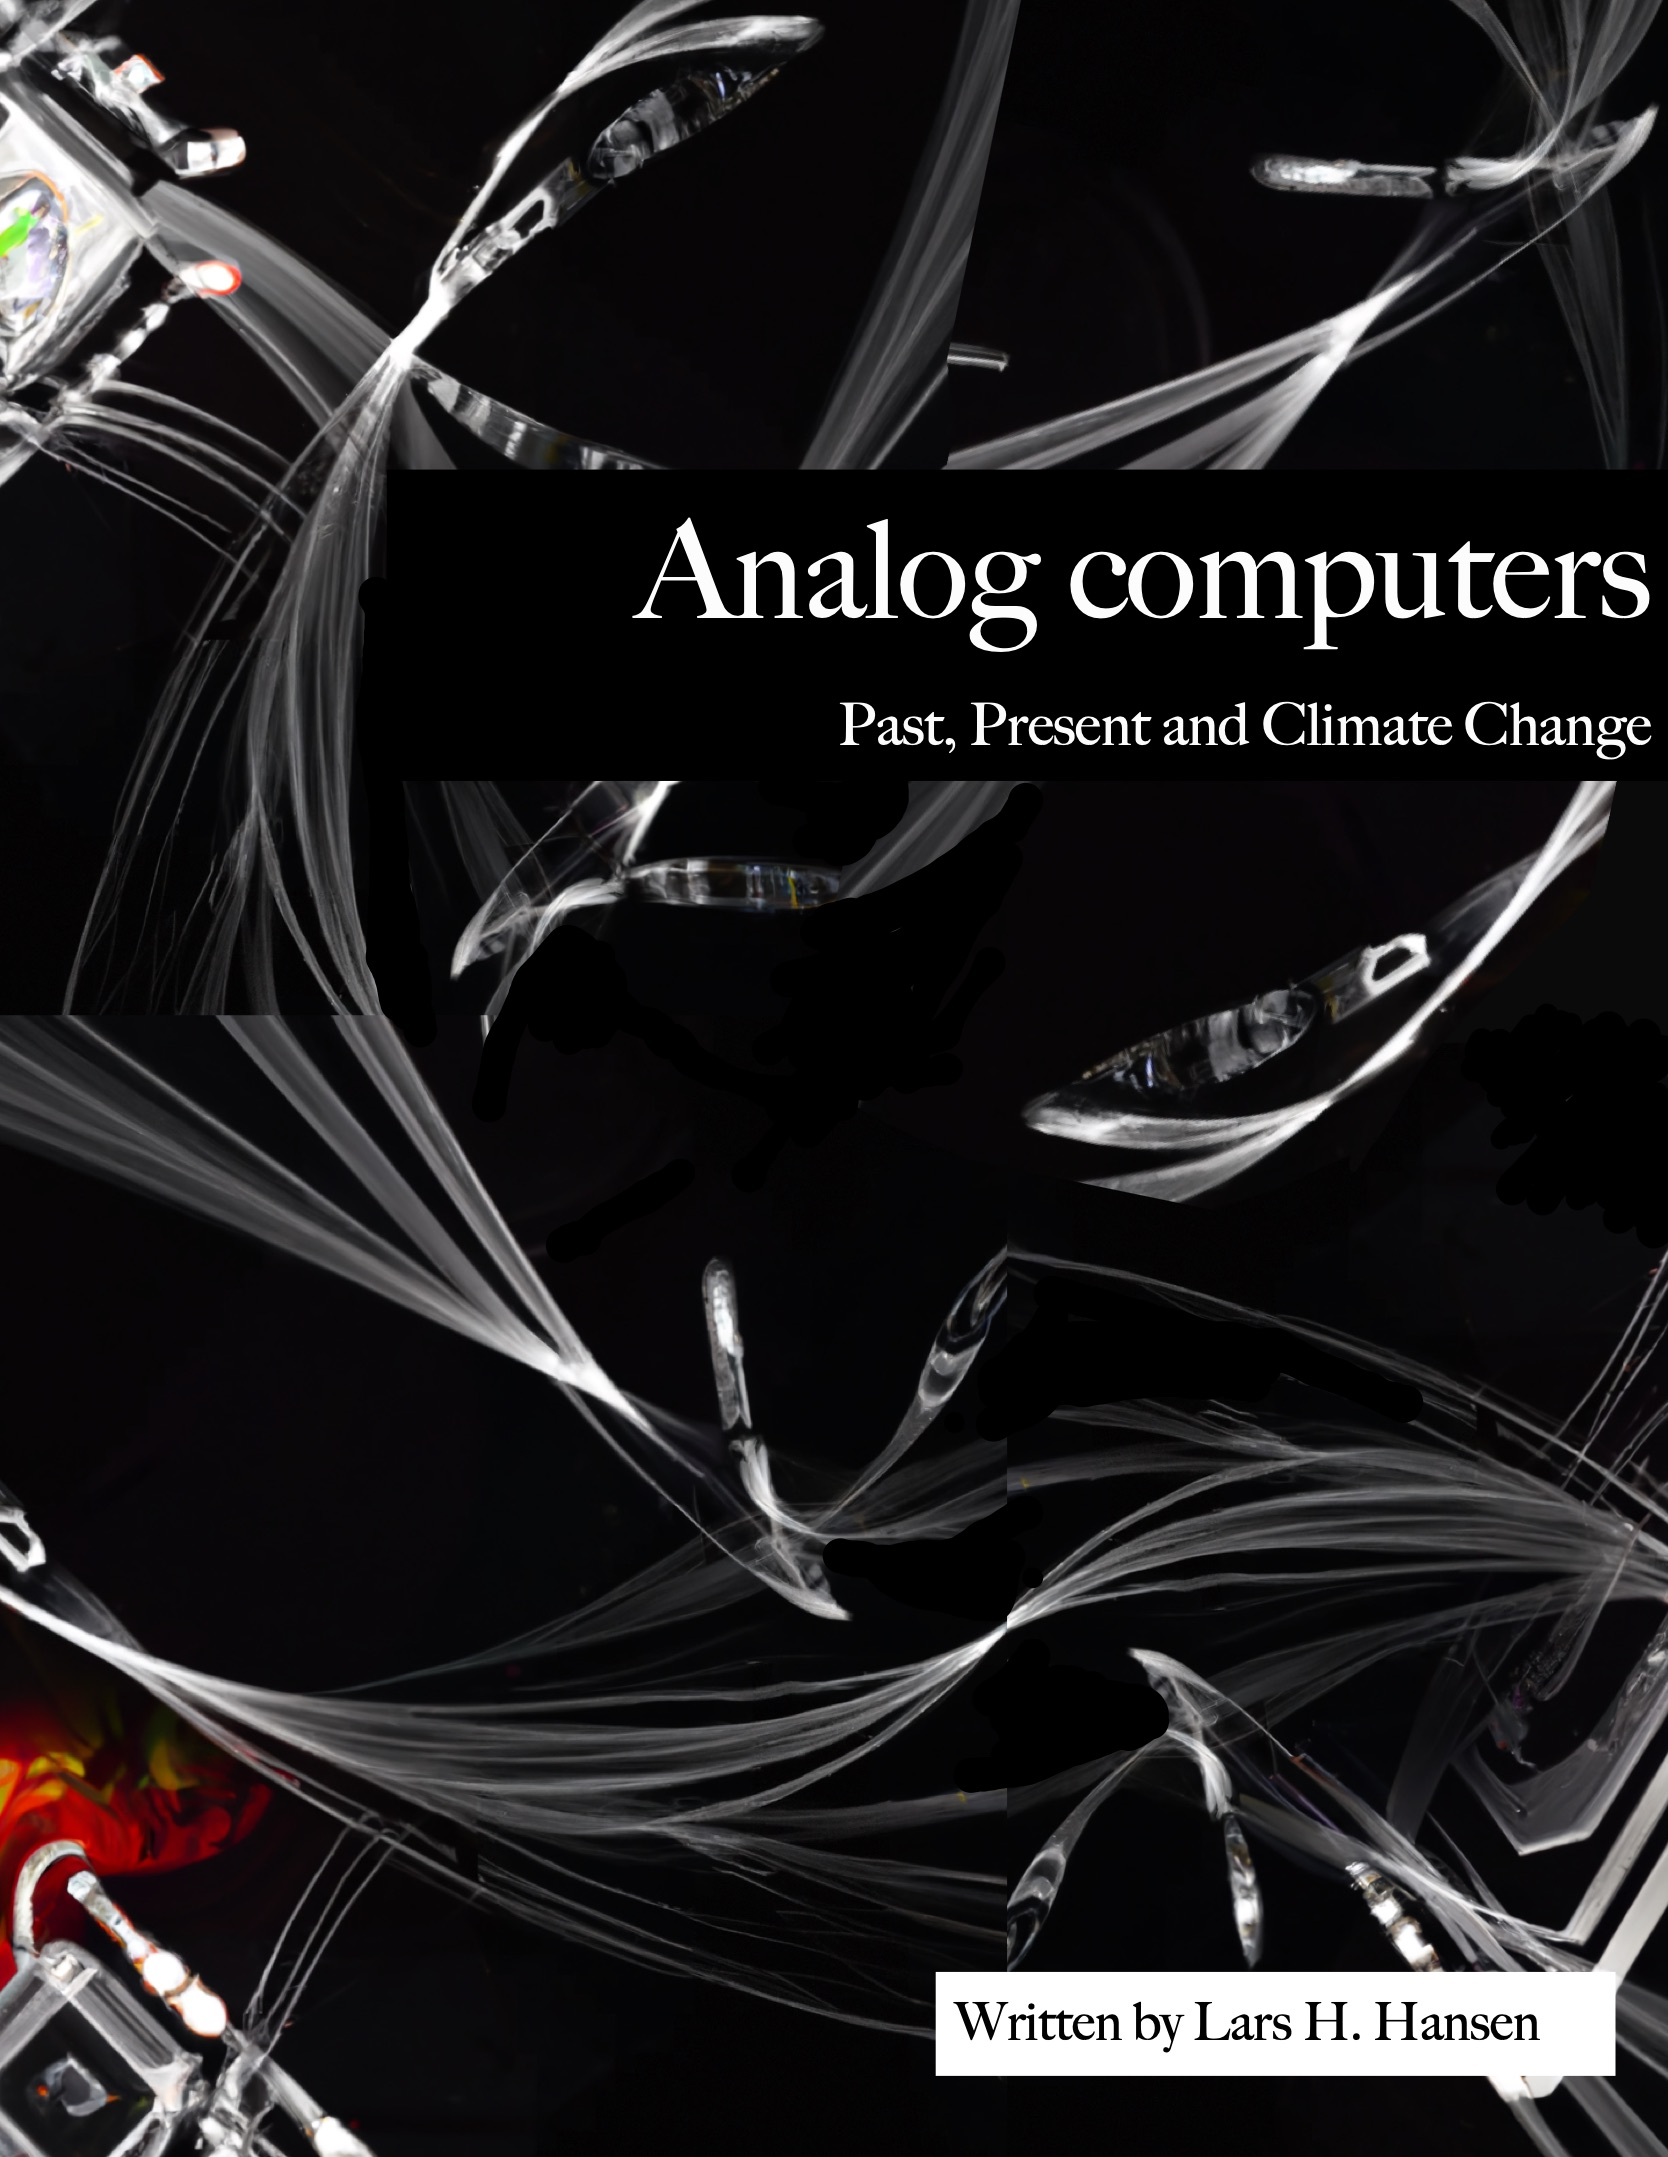
\includegraphics[scale=0.4]{ACPPCbookCover.jpg}
\pagestyle{classicbookstyle} % Apply the custom page style


\newpage
\maketitle
\tableofcontents
\newpage
\Large{Thanks to}\\
Thank to my friends and family for supporting me while writing this book. Thans to Simon Walsh and Ryan Furgesson from my highschool AISJ in South-Africa for teaching me and inspireing me to pursue a carrer in STEM. 

Thank you Lars Magne Lundheim, profesor at ELSYS at the Norwegian University of Science and Technology (NTNU) for being so incredibly pedagogical and inspireing. Thank you also for the academic support and guidence while writing this book. This book would be not exist without you. 

Thank you also to Erik Folven at NTNU for caring to such a great extent for youre students. 

Thank you OrbitNTNU :D What a great group of people you guys are. Im glad to be a part of the satellite team. \lipsum[1]

\newpage
\Large{Introduction}\\
\lipsum[1-2]ffF

\chapter{The Analoge Renesance}
Since the beginning of mankind, compute has been a vital part of both survival and wellbeing. 
Being able to deduct new and usefull information from observation has allways been important. 
It would for example be usefull to estimate how much wood was needed in order to keep a fire burning through the nigth.
Or how many times you could repeat the same tune before your friend gets annoyed at you.

As we all know: human are lazy. We have thoroughout our history worked on externalizing ourselves. Burning food on fires instead of processing the food in our stomach. Planting seeds and farming animals instead of hunting, whatch other people play sports instead of doing it ourselves and so on... 

This naturally applies to computing as well. And it is so damn cool!

Allthough in recent years computing has not really been so cool. Due to quantum effecs such as electrontunneling leading to leakage current in transistors, heat is generated. This heat is proportional to the clockspeed of the specific chip. This poses several issues to modern computing. First of all it limits the shrinking of transistors. Second, it leads to computers having to be constantly cooled down by external hardware. Furthermore the size of a digital tranistor is reaching its physical possible size. The size is literally more and more comparable to the size of atoms.

But what kind of computing could possibly exeed these boudaries? Hard to tell... Especially when the title of this book doent even give one hint to what type of cumputing this could be.


\section{Predicting the tides}
In xxxx mr ??? used the ??? in order to predict the tides...
This was namely very usefull information for ships at the time. When coming in to dock it was usefull to know what the heigth of the water would be etc... ???

\chapter{Analoge Computing Principles}
\section{Addition}
Kirshov current law
\section{Multiplication}
Voltage dividers
Transistors
\section{Integration}
The mechanical integrator
\section{Division}
\section{Derivation}
\section{Accuracy and noise}
In comparison to the modern digital cirquits; analog stuff can be quite noisy. 
However, that is not neccecarily a downside.
\subsection{Electromagnetic interferance}
\subsection{Varing conductivity}
\subsection{Temperature}
\section{Artificial Spin Ice!}
Artificial Spin ice (ASI) are, unlike most other man made systems, a mixture of both computation and storage.
This unique quality is made possible by using a system of coupled magnets

\chapter{Applications}
\section{Ai training and modeling}
\section{Simulating complex systems}
\section{Simulating the brain}

\chapter{Analouge and Digital Synergy}
\section{Addition}
Kirshov current law
\section{Multiplication}
Voltage dividers
Transistors
\section{Integration}
The mechanical integrator
\section{Division}
\section{Derivation}
\section{Accuracy and noise}
In comparison to the modern digital cirquits; analog stuff can be quite noisy. 
However, that is not neccecarily a downside.
\subsection{Electromagnetic interferance}
\subsection{Varing conductivity}
\subsection{Temperature}
\section{Artificial Spin Ice!}
Artificial Spin ice (ASI) are, unlike most other man made systems, a mixture of both computation and storage.
This unique quality is made possible by using a system of coupled magnets

\chapter{Future Prospects}
The end of moores law


\chapter{Conclusion}
In conclusion

\appendix{Work Cited}

\newpage
\appendix{Appendix A}

\end{document}
